\begin{problem}%
{Драконий язык}%
{\textsl{стандартный ввод}}%
{\textsl{стандартный вывод}}%
{1 секунда}%
{64 мегабайта}{}

\begin{center}
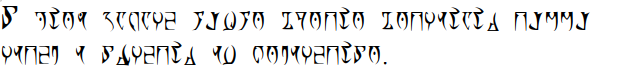
\includegraphics[scale=0.8]{images/daedric.png}
\end{center}

\InputFile

В первой строке вводится целое число $N$ ($0 \le N \le 10^4$). В следующей строке вводятся $N$ целых чисел, каждое из которых по модулю не превышает $10^4$, разделённых пробелами.

\OutputFile

Выведите ответ на задачу.

\Examples

\begin{example}
\exmp{
2
1 2
}{%
1
}%
\end{example}
\end{problem}
